\subsection{BOLD data}
For image data, we did several explanatory data analysis to better under the 
BOLD data. 
\begin{itemize}
\item Reproduce Quality Assurance(QA) plots\\
 We reproduced some of the QA Plots provided in the BOLD folder, including 
 mean signals, Framewise Displacement and DVARS(root mean squared signal 
 derivative over brain mask). The shapes were almost the same, except the y 
 axis. We assumed there was some transformation or preprocessing in the 
 original QA plots.
\item Correlation \\
 We calculated the correlation between task-on/task-off vectors and voxel time 
 courses to identify the active region of the brain. Below is an example of correlation figure of the middle slice in subject 1.\\
  \begin{figure}[H]
    \centering
        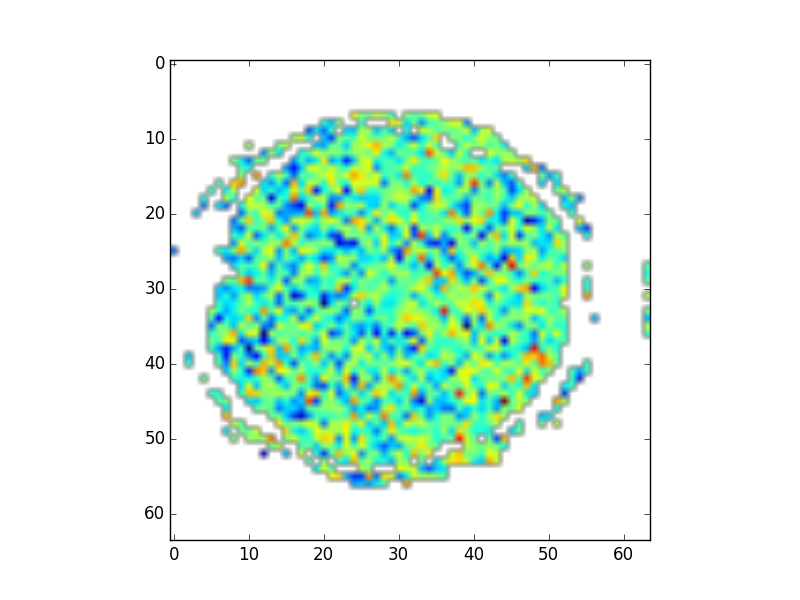
\includegraphics[scale=0.5]{correlations.png}
    \caption{Correlation between On/Off and Voxel Time Course}
\end{figure}
\item Associated the brain image data with behavior data\\
We started to associate brain image data(mean/standard deviation across time courses) with gain/loss/ratio, choices(accept/reject) and respcat(strongly/weekly accept/reject).
\end {itemize}
